\chapter{Arquitectura del sistema}  \label{arquitectura_sec}
\section{Flujo de trabajo}  \label{workflow_subsecc}

Describiremos el diseño confeccionado en detalle. Se tienen tres etapas fundamentales:

\begin{itemize}
\item \textbf{Pre-procesamiento:} consiste en capturar la imagen aplicando las
  transformaciones mencionadas en la sección \ref{dynamicrange} y \ref{fixedpoint}, empleando un script hecho en Python. Este script divide la imagen en lotes o batches y los envía a la FPGA, a través del puerto UART. Un batch o lote, consiste en columnas contiguas de pixeles cuya dimensión se explica en la sección x.
    %% Poner seccion aca
\item \textbf{Procesamiento:}	: el batch es convolucionado con el kernel dentro del módulo. Dicho kernel es configurable, y el usuario puede cargar los coeficientes del mismo mediante el GPIO. 
  Cuando la operación de la convolucion finaliza, una notificación es enviada a
  un microprocesador en la FPGA, que da la orden de recuperar el batch procesado, para así enviarlo a la unidad central de procesamiento (CPU).
\item \textbf{Post-procesamiento:}Como etapa final, en el post-procesamiento se combinan los batches o lotes en CPU usando el script de Python.
\end{itemize}

\section{Estados y transiciones}  \label{states_subsecc}

\begin{figure}
\centering
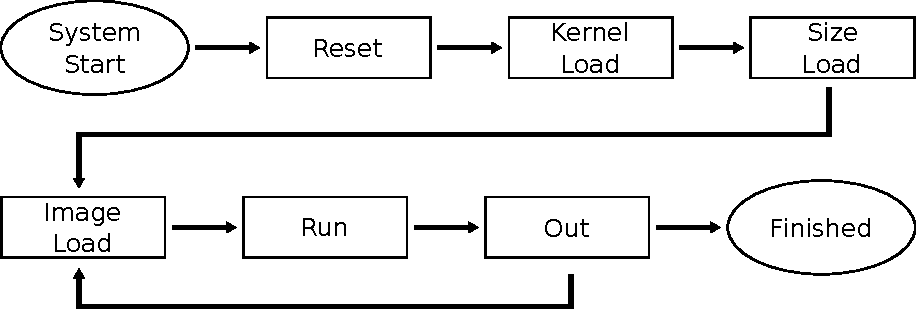
\includegraphics[scale=0.7]{states.pdf}
\caption{Diagrama de estados del sistema.}
\label{statesfig}
\end{figure}

El módulo atraviesa distintos estados para llevar a cabo su tarea. Estos estados
se pueden observar en la figura~\ref{statesfig}.

La transición entre un estado y
otro se realiza mediante instrucciones codificadas en el frame de entrada de 32
bits asentado en el GPIO. El módulo permanece en su estado actual hasta recibir
una instrucción valida.

Inicialmente, debe situarse al sistema en un estado de reset, y por ende debe
recibir una señal de reset para establecerse en dicho estado, esperando a ser
configurado.
Luego de recibir la correspondiente instrucción, se produce una transición hacia el estado KernelLoad, en donde los coeficientes del kernel se cargan al módulo.
El siguiente estado (SizeLoad), es en el cual se carga el tamaño de la imagen,
más precisamente la altura de la misma, esto permitirá conocer la posición del
último dato en memoria.
Estos tres estados mencionados, solo se ejecutan una vez durante todo el ciclo
de trabajo. El proceso se repite por cada nueva imagen, por ende, si se desea
procesar una nueva imagen, inicia el ciclo nuevamente.

Pasada la etapa de carga, la primera transición es hacia el
estado ImageLoad, donde se almacena el lote en la Block RAM de la FPGA.
Teniendo el lote almacenado, la transición luego es hacia el estado run donde se
hace el filtrado del lote, y mientras el sistema se situe en este estado, no
puede ser interrumpido.
Como consecuencia, cualquier instrucción recibida se ignora hasta que se
complete esta etapa de procesamiento de lote.

Cuando se finaliza el procesamiento de un lote, se emite una notificación y el sistema
queda en espera de la última señal para pasar hacia el estado Out. Una vez recibida la
correspondiente instrucción codificada, se devuelve el lote procesado al
microprocesador de la PC.

\begin{figure}
\centering
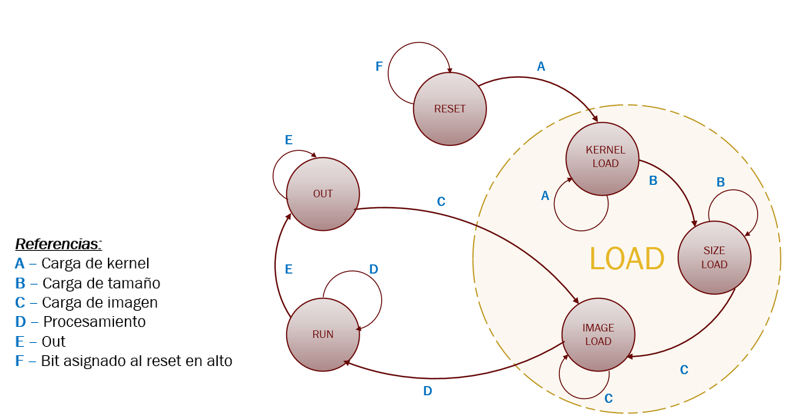
\includegraphics{states_2.png}
\caption{Diferentes estados y las etapas involucradas }
\label{statesfig2}
\end{figure}

\section{Arquitectura del módulo de convolución}  \label{ourdesign_subsecs}

El diseño planteado prioriza la reutilización dinámica de memoria, en donde por
cada iteración en la etapa de procesamiento, se aprovecha la disponibilidad de
datos cargados en memoria en la iteración anterior.
En la figura~\ref{general}, se muestran los bloques principales que conforman el
diseño. Los bloques que integran el módulo son:

\begin{figure}
\centering
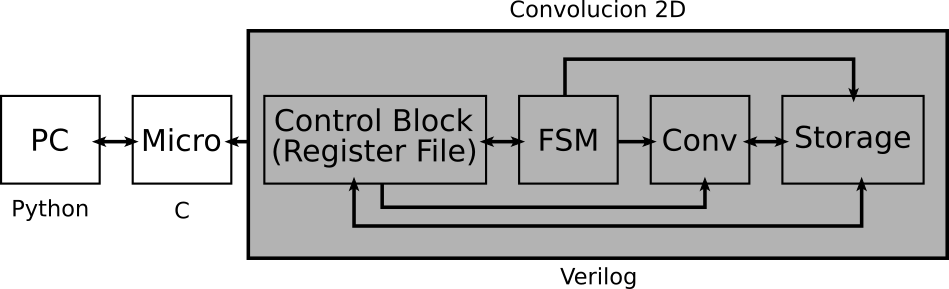
\includegraphics{general}
\caption{Arquitectura general del sistema }
\label{general}
\end{figure}

\begin{itemize}
\item \textbf{Control Unit:} se encarga del manejo de la comunicación entre el
  módulo y el procesador instanciado en la FPGA.
\item \textbf{MAC Unit -Multiplier-ACcumulator:} ejecuta la suma de los productos entre los coeficientes del kernel y los pixeles de la imagen. 
\item \textbf{Address Generation Unit (AGU):} bloque que maneja las direcciones
  de memoria que deben ser leídas o escritas.
\item \textbf{Storage:} hace referencia a un conjunto de columnas formadas por
  BRAMs de la FPGA. El tamaño depende de la cantidad de MACs instanciadas,
  o en otras palabras, el paralelismo a nivel de cantidad de convoluciones en
  paralelo, que se desee en el sistema.
\end{itemize}
%TODO: falta MMU
     
Estos bloques se describen en mas detalle en las secciones siguientes.

\subsection{Control Unit}\label{sec:ctrl_u}
El bloque Control Unit es el encargado de hacer de interfaz entre los bloques
restantes del módulo de convolución y el microprocesador que se encuentra en la
FPGA. Para hacer esto, cuenta con dos puertos de 32 bits conectados a los GPIO
de entrada y salida del procesador.

El bloque interpreta las instrucciones que recibe y modifica las señales de
control conectadas a los otros bloques, esto representa la transición de
estados mencionada en la sección~\ref{states_subsecc}.

La organización del frame de entrada de 32 bits, junto con los códigos binarios
de las instrucciones se muestra en la tabla~\ref{instr}.

\begin{table}
% increase table row spacing, adjust to taste
\renewcommand{\arraystretch}{1.3}
% if using array.sty, it might be a good idea to tweak the value of
% \extrarowheight as needed to properly center the text within the cells
\caption{Código de instrucciones, la letra 'd' representa bit de datos.}
\label{instr}
\centering
% some packages, such as mdw tools, offer better commands for making tables
% than the plain latex2e tabular which is used here.
\begin{tabular}{|l|c|c|c|c|c|}
  \hline
  \multicolumn{1}{|c|}{\multirow{2}{*}{\textbf{Instrucción}}} & \multicolumn{5}{c|}{\textbf{BITS}} \\ \cline{2-6}
                                        & \textbf{31 - 29} & \textbf{28 - 25} & \textbf{24 - 14} & \textbf{13 - 1} & \textbf{0}\\\hline
  Cargar kernel                         & 000              & xxx              & ddddddddddd      & ddddddddddddd   & 0         \\\hline
  Cargar tamaño imagen                  & 001              & xxx              & xxxxxxxxxxx      & xxxdddddddddd   & 0         \\\hline
  Cargar lote                           & 010              & xxx              & xxxxxxxxxxx      & ddddddddddddd   & 0         \\\hline
  Recuperar dato                        & 011              & xxx              & xxxxxxxxxxx      & xxxxxxxxxxxxx   & 0         \\\hline
  Finalización de lote                  & 100              & xxx              & xxxxxxxxxxx      & ddddddddddddd   & 0         \\\hline
\end{tabular}           
\end{table}

Como el módulo y el procesador trabajan a distintas frecuencias de reloj, se
puede producir un error al enviar y recibir datos entre ambos. Para superar este
problema, el flanco ascendente del bit 28 se utiliza como indicador de que un
nuevo dato esta listo para ser leído o escrito. 

El bit 0 se utiliza como indicador del estado del módulo, en caso de ser 1 el
módulo se pone en estado de reset, por lo que una vez atravesado este estado,
siempre debería permanecer bajo.

Las instrucciones cumplen las siguientes funciones:

\begin{itemize}
\item \textbf{Cargar kernel:} Se utiliza para cargar los coeficientes del
  kernel, cada coeficiente es de 8 bits, junto con la instrucción se deben
  añadir los 3 coeficientes que forman una columna del kernel.\footnote{Para un
    diseño que utiliza kernels de $3\times3$, en caso de ser de dimensiones
    superiores, nuevas instrucciones deben ser añadidas.}
\item \textbf{Cargar tamaño imagen:} A esta instrucción debe acompañar el tamaño
  del alto en pixels de la imagen, se utilizan 10 bits para ello por lo que el
  tamaño máximo es de 1024px.
\item \textbf{Cargar lote:} Instrucción que indica que los datos corresponden a
  un pixel del lote.
\item \textbf{Finalización de lote:} Indica que el pixel que se esta cargando es
  el último pixel del lote, una vez recibida esta instrucción el módulo pasa al
  estado de run donde realiza el procesamiento.
\item \textbf{Recuperar dato:} Con esta instrucción se pide al módulo que
  entregue el pixel procesado siguiente.
\end{itemize}

Como se nombró anteriormente, una instrucción no será considerada hasta que no
haya un flanco ascendente en el bit 28.

\subsection{Address Generator Unit (AGU)}

El AGU es el encargado de generar las direcciones de memoria que son
consumidas por el MMU.

Durante el estado de ImageLoad, el AGU genera las direcciones donde se deben
escribir estos datos, para ello cuenta con un contador que se incrementa con
cada flanco de subida del bit 28 de la entrada del Control Unit
(sección~\ref{sec:ctrl_u}). El AGU además conoce el alto de la imagen (cargado
durante SizeLoad) por lo que una vez que el contador alcanza dicho valor envía
una señal al MMU indicando que el pixel que se recibe a continuación pertenece a
una nueva columna del lote.

Durante la etapa de procesamiento el AGU debe producir dos direcciones
diferentes, una que indica al MMU los datos que debe entregar a las unidades MAC
y otra que indica al MMU la posición donde los datos procesados por las MACs
deben ser almacenados. Ambas direcciones se incrementan una vez por ciclo de
reloj, pues las MAC generan un dato procesado por ciclo. La diferencia entre la
dirección de lectura y la dirección de escritura es igual a la latencia que
existe desde que se entrega el primer pixel a una unidad MAC hasta que el primer
pixel procesado este listo para almacenarse.

Durante el estado Out, o de salida de datos, el AGU genera las direcciones de
lectura de los datos procesados, al igual que en el estado de ImageLoad, se
incrementa con cada flanco de subida del bit 28 y tiene en cuenta el alto de la
imagen para hacer el cambio de columna de datos.

% \subsection{Multiplier Acumulator Unit (MAC)}

% \subsection{Memory Management Unit (MMU)}

% \subsection{Storage}
\subsection{Almacenamiento}\label{storage_subsecc}
Los coeficientes del kernel se almacenan en registros dentro de cada MAC Unit.
Para almacenar un lote, el enfoque que se opto fue organizar la BRAM en
columnas. Cada columna entonces, corresponde a una columna del lote.

El tamaño del lote está dado por la altura de la imagen y por el número de
columnas de memoria instanciadas.  La máxima altura en pixels de la imagen,
entonces, debe ser menor o igual al número de direcciones de una columna de
memoria instanciada.

Durante el procesamiento del lote, cada pixel se lee únicamente una vez, lo que permite un uso mas eficiente de la memoria. Los pixeles que ya se utilizaron, se sobrescriben con los pixeles procesados. 
Esto permite reducir la cantidad de memoria necesaria, ya que reúsa la misma memoria para almacenar el lote de entrada, y el lote procesado.

\subsection{Procesamiento de datos}  \label{processing_subsecc}
Para un kernel de  $(k \times k)$, cada MAC Unit toma $k$ columnas de memoria
adyacentes como entrada.

El bloque $MAC$  $Unit$ necesita primero que se carguen k pixeles de cada
columna para asi tener $(k \times k)$ pixeles cargados dentro de ella para así
producir el primer pixel procesado.

Luego, se procede a efectuar la multiplicación de los pixeles con los coeficientes del kernel y sumar cada termino.

Finalmente se trunca el resultado, y se almacena el mismo en la primera posición de memoria.

Una vez que se procesa un pixel, se almacena en la memoria mientras bloque $MAC$  $Unit$ efectua un desplazamiento (shift) de sus registros en donde se almacenan pixeles de la imagen, para asi descartar los k pixeles mas antiguos,
 y se cargan los $k$ nuevos pixeles, es decir, uno de cada columna de entrada, lo que es equivalente a una estructura FIFO (First Input – First Output).
Se sincroniza lo mencionado anteriormente de forma tal de obtener un pixel por cada ciclo de clock.

Este procedimiento es equivalente a desplazar verticalmente el kernel sobre la imagen:

\begin{figure}
\centering
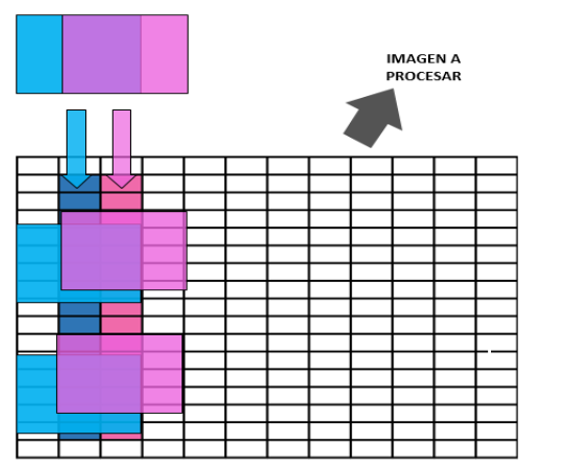
\includegraphics[scale=0.7]{conv1_despl.png}
\caption{Desplazamiento vertical del kernel sobre la imagen }
\label{verticaldesp}
\end{figure}


El módulo $AGU$ maneja las direcciones de memoria, tanto lectura como de escritura, teniendo en cuenta la latencia desde que un pixel se carga en bloque $MAC$ $Unit$ hasta que el pixel procesado correspondiente sea almacenado.
Todo lo mencionado anteriormente fue de manera genérica sobre una sola MAC Unit, pero ahora se explicara como poder trabajar en el sistema con mas de uno de estos modulos instanciados en paralelo:

\begin{itemize}
\item Como se mencionó,  se necesitan $k$ columnas como entrada para producir una columna procesada en una $MAC$ $Unit$. Por lo tanto, $2 \times k$ columnas, se necesitan para $2$ $MACs$.
\item Debido a la naturaleza de la operación de la convolucion, para obtener una columna contigua, se necesita desplazar una vez las columnas de entrada. Entonces, existe un solapamiento entre 2 de las entradas de las MACs que producen columnas adyacentes, y así la información puede ser compartida.
  Así, pese a necesitar $k$ columnas de entrada por cada unidad $MAC$, solamente $k+1$ columnas diferentes de entrada se necesitan para dos $MACs$ instanciadas.
\item Entonces, para $N$ $MACs$, el número requerido de columnas de memoria, se reduce de $N \times k$ a $N+k-1$, concluyendo que agregar una nueva unidad $MAC$ solamente agrega una nueva columna de memoria.
\item Debido al solapamiento explicado anteriormente, hay información repetida entre un lote recibido y el siguiente, por lo que, para reducir la transmisión de datos, esta información repetida se mantiene en memoria y solamente se transmite la parte faltante del lote entrante.
Dadas $N$ $MACs$ y  un kernel de $k \times k$, un lote cuyo ancho (o cantidad de columnas) sea de $N+k-1$ es necesario. No obstante, el lote procesado tendrá un ancho de  $N$ columnas, es decir, una por unidad $MAC$, por lo que las ultimas $k+1$ memorias no se sobrescriben y mantienen los datos de entrada. Estas $k+1$ columnas se reutilizan como las primeras columnas del siguiente lote, y asi, el ancho del lote transmitido se reduce a $N$, con la excepción de que el primer lote mantiene un ancho de $N+k-1$.
\end{itemize}

La reutilización de columnas de memoria escritas por los lotes previos, resulta en un desplazamiento circular en $N$ lugares, desplazando la posición de las columnas de memoria asociadas con cada unidad $MAC$ en cada iteración.De lo anterior, se deduce que existe una periodicidad entre la relación de columnas de memoria y las entradas de las unidades $MAC$, donde el periodo It es el número de iteraciones necesario para obtener la relación ente las columnas de memoria originales con respecto a las entradas de las unidades $MAC$.
Entonces, matemáticamente: Cuando $It(k-1)$ es un múltiplo de $N+k-1$, debe existir un numero entero $m$, tal que:

\begin{equation}\label{niter}
  \frac{It}{m} = \frac{N}{k-1} + 1
\end{equation}

Sintetizando el algoritmo descrito, dadas $N$ $MACs$ y  un kernel de $ k \times k$:

\begin{itemize}
\item Lote de imagen sin procesar,  con $N+k-1$ columnas es necesario
	\item El lote procesado tendrá un ancho de $N$ columnas
	\item Las ultimas $k+1$ memorias no se sobrescriben
	\item Estas $k+1$ columnas se reutilizan como las primeras columnas del siguiente lote
	\item El ancho del lote transmitido se reduce a $N$, con la excepción de que el primer lote mantiene un ancho de $N+k-1$.
	\item Sea el periodo $It$  el número de iteraciones necesario para obtener la relación ente las columnas de memoria originales con respecto a las entradas de las unidades $MAC$.
	\item Cuando $It(k-1)$ es un múltiplo de $N+k-1$, existe un numero entero $m$, tal que:
\begin{equation}
  \frac{It}{m} = \frac{N}{k-1} + 1
\end{equation}
\end{itemize}

Veamos las ventajas del diseño planteado de forma gráfica:

\begin{figure}
\centering
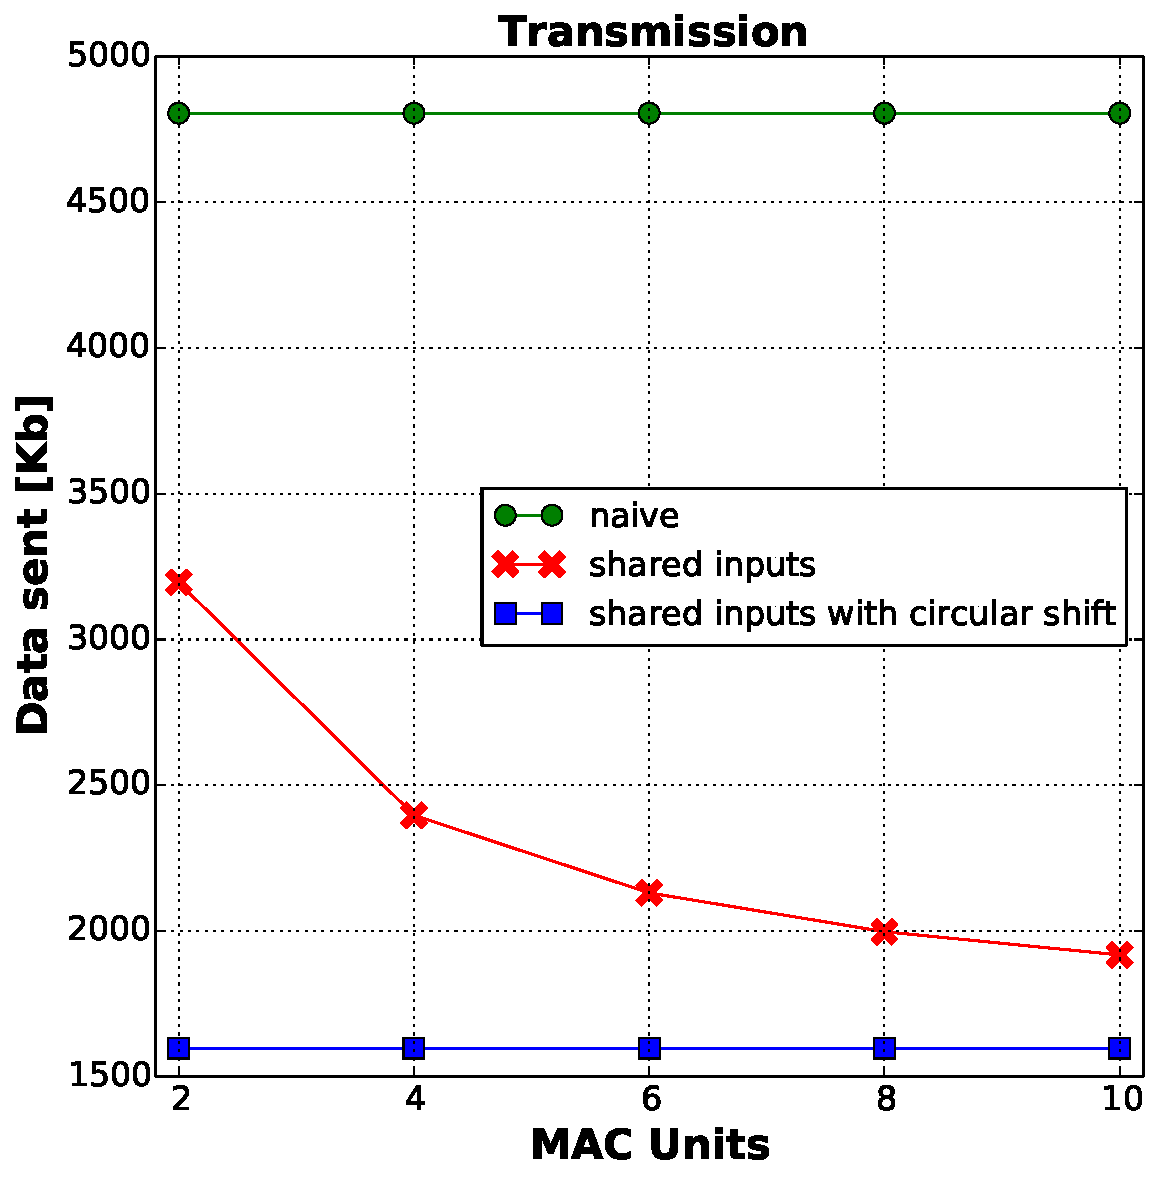
\includegraphics[scale=0.5]{data_sent}
\caption{Cantidad de memoria requerida en función del grado de paralelismo }
\label{memoryrequired}
\end{figure}

\bigskip
Se ve en la figura que a medida que se instancian más unidades $MAC$, o en otras palabras, a medida que se aumenta el grado de paralelismo del sistema haciendo referencia a la cantidad de convoluciones en paralelo con las que se trabaja, el primer enfoque propuesto requiere mucha mas memoria para operar que el enfoque de información compartida, donde se reutilizan ciertas columnas dada por la matemática y relaciones descritas.\\

\bigskip
\bigskip
Por otra parte, para lo que refiere a la transmisión, se tiene:

\begin{figure}
\centering
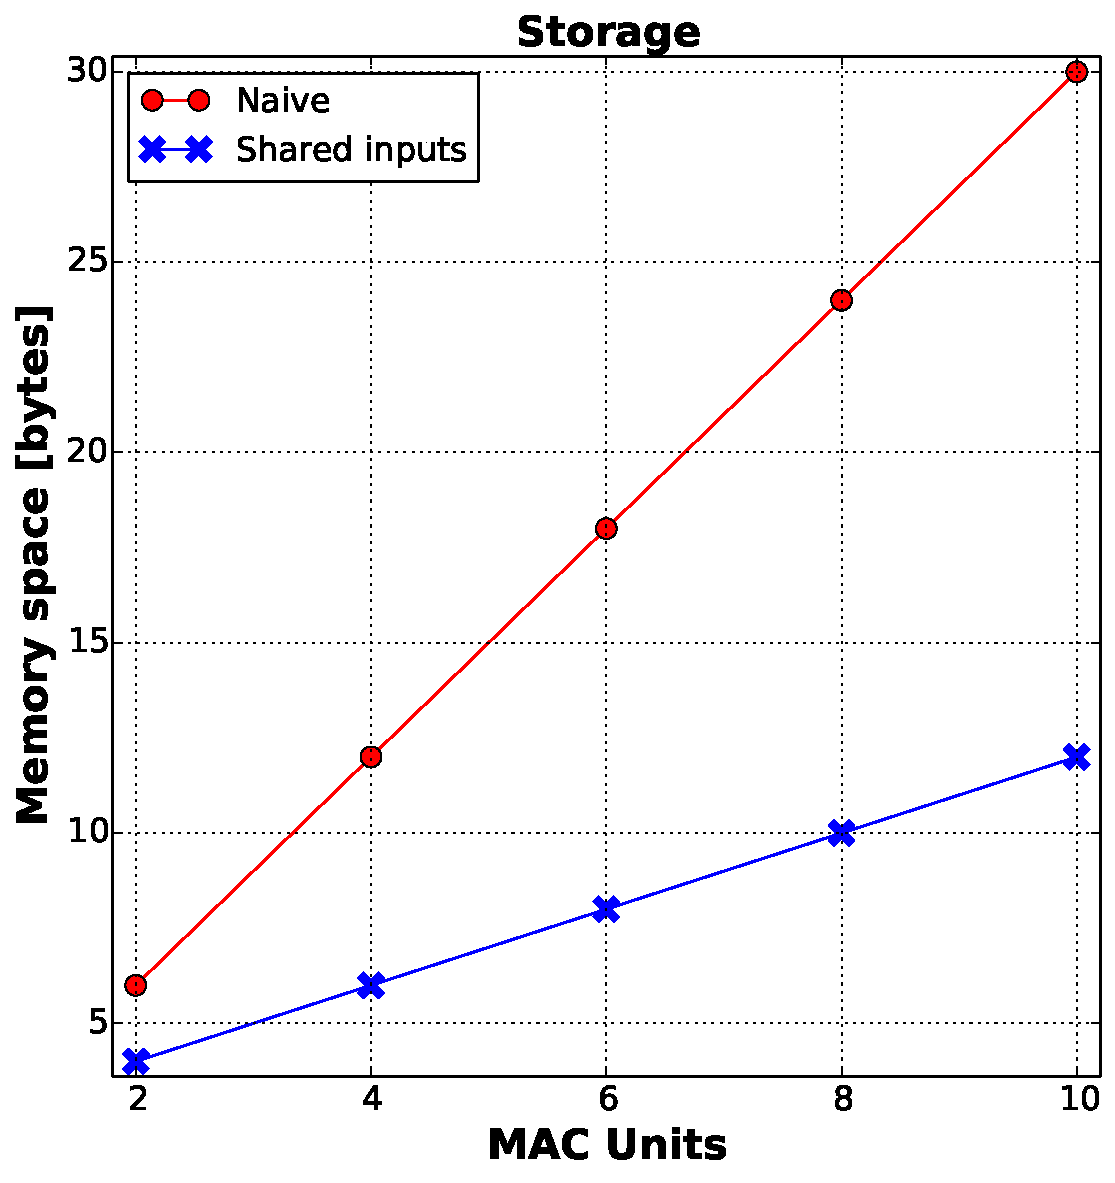
\includegraphics[scale=0.5]{mem_space2}
\caption{Transmisión de datos en función de unidades MAC instanciadas }
\label{datatransmision}
\end{figure}

Se mencionó que, debido al solapamiento, hay información repetida entre un lote recibido y el siguiente, por lo que, para reducir la transmisión de datos, esta información repetida se mantiene en memoria y solamente se transmite la parte faltante del lote entrante.\\

En la figura se muestra como el diseño planteado con el desplazamiento circular requiere una transmisión constante notablemente menor a comparación del primer enfoque que se planteo, y como también el hecho de reutilizar la información compartida tiende a una disminución en la transmisión de datos durante el funcionamiento del sistema. La imagen con la que se efectuaron las gráficas tenía un tamaño de $1600 \times 1024$.

\bigskip
\bigskip
\bigskip

\subsection{Proceso de escritura en memoria}  \label{writing_subsecc}
\smallskip
Se analiza el caso de tener instanciadas $N=4$, $MACs$ y un kernel con $k=3$ para clarificar la operación del algoritmo descrito.
El proceso de escritura en memoria, utilizando el desplazamiento circular de columnas mencionado.\\

Como consideramos un kernel con $k=3$ y $N=4$, $MACs$:
\begin{frame}{}
	    
      \begin{itemize}
        \item Se necesitan o requieren N+k-1=4+3-1=6 columnas de memoria
	\item En la primera iteración, se cargan las memorias 1 a 6 con el nuevo lote (donde cada memoria instanciada alberga una columna del lote) y el resultado se almacena en las memorias 1 a 4, marcadas con otro color y en la etapa run  out.
	\item En la segunda iteración, los datos del nuevo lote se cargan sin sobrescribir las memorias 5 y 6 . Luego del procesamiento, se almacenan los datos comenzando en la memoria  5 hasta la última, para luego sobrescribir los datos del lote previo desde el principio.

\bigskip
\bigskip
Lo anterior se puede apreciar en la siguiente figura, donde se incluye una línea punteada que separa la etapa de carga y la de procesamiento y salida de dato:

\end{itemize}
\end{frame}

\begin{figure}
\centering
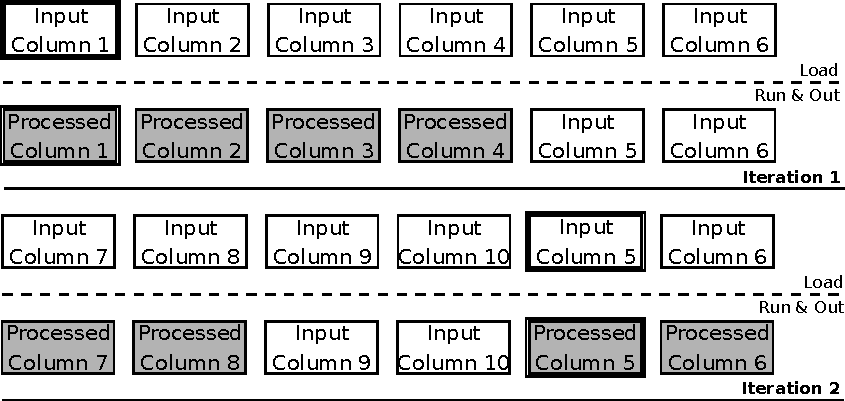
\includegraphics[scale=0.8]{algorithm}
\caption{Algoritmo de escritura para N=4, k=3 }
\label{writingprocess1}
\end{figure}

Considerando ahora un kernel con $k=3$ y  $N=2$, $MACs$, se anexan graficos para ilustrar lo mencionado de forma mas clara, 
donde se distinguen con colores las columnas involucradas y las etapas respectivas:

\begin{figure}
\centering
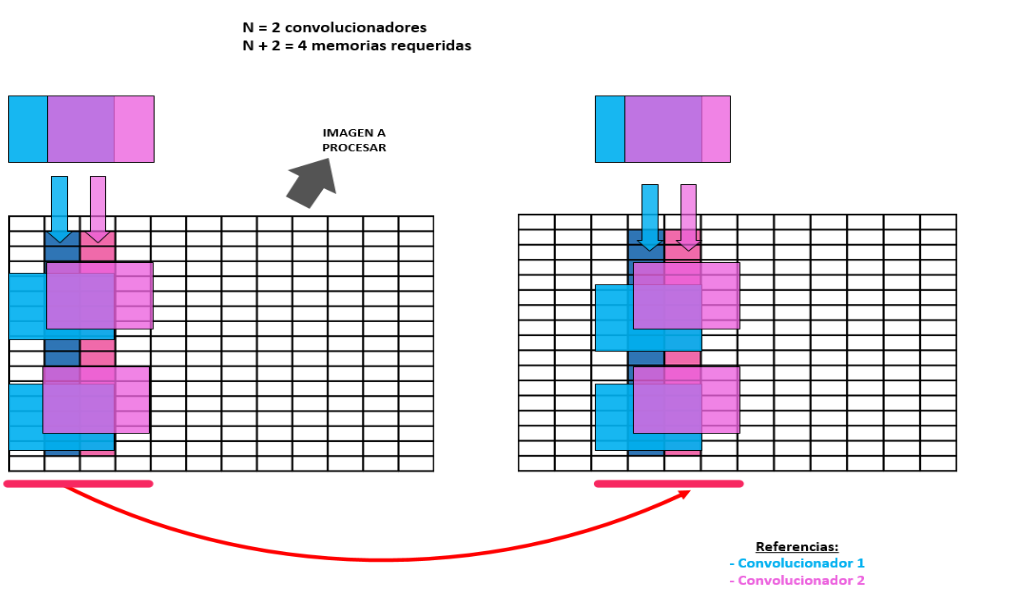
\includegraphics[scale=0.75]{conv2_despl.png}
\caption{Desplazamiento del kernel paraa N=2, k=3 }
\label{writingprocess2}
\end{figure}

\begin{figure}
\centering
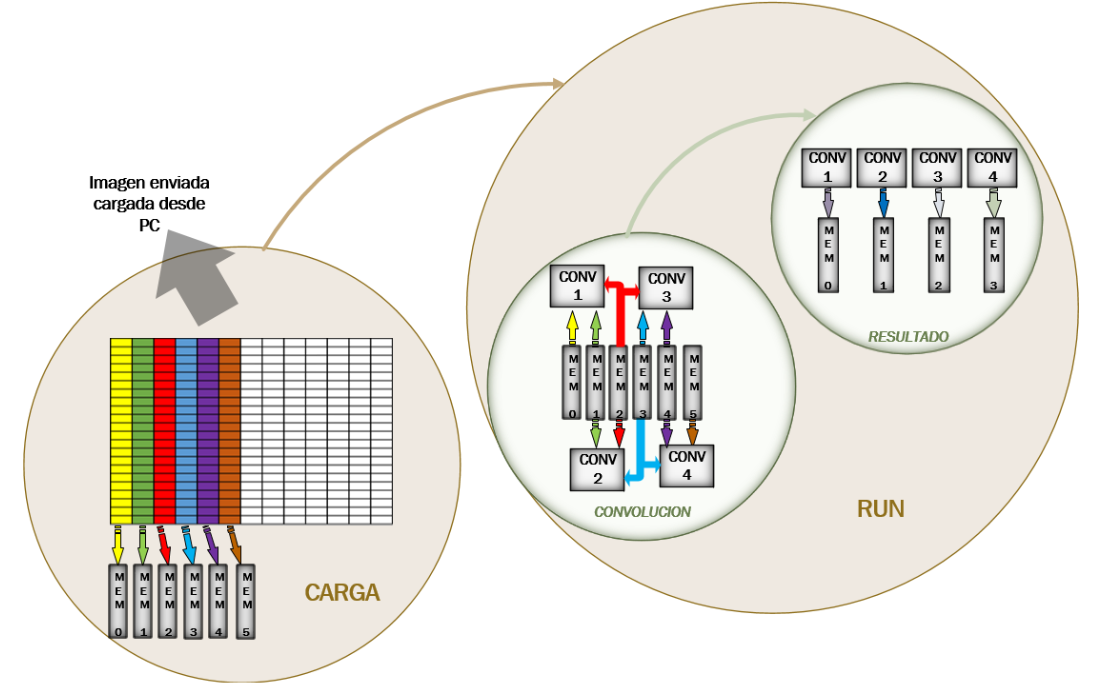
\includegraphics[scale=0.7]{example_1}
\caption{Primera iteración con N=2, k=3 }
\label{writingprocess3}
\end{figure}


\begin{figure}
\centering
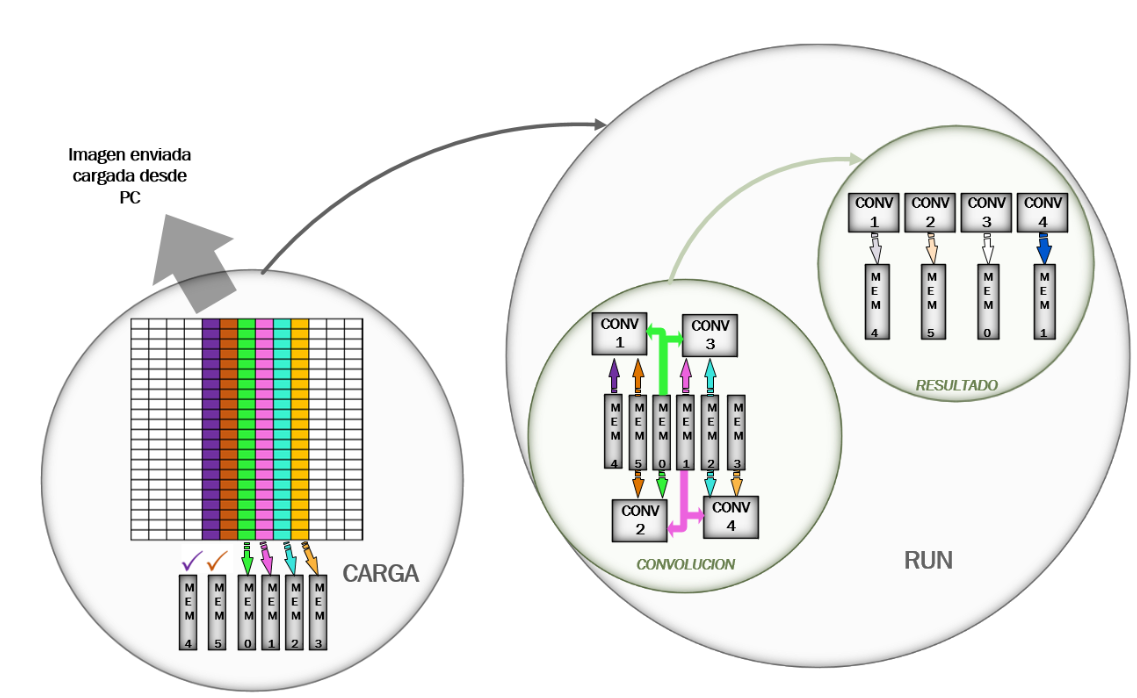
\includegraphics[scale=0.7]{example_2}
\caption{Siguiente iteración con N=2, k=3}
\label{writingprocess4}
\end{figure}




La lógica del sistema se implementa en el bloque $MMU$ ($Memory$ $Managment$ $Unit$), que sirve como interfaz entre las memorias y el resto de los componentes, 
manteniéndolos independientes al grado de paralelismo del sistema y al número de iteración.

\bigskip

\section {MMU (Memory Managment Unit) }  \label{mmu_subsecc}
Este bloque, en cada iteración, mantiene un seguimiento de las posiciones de memoria donde el lote entrante debe ser almacenado,
la información que debe alimentar a cada unidad $MAC$, lLa posición de memoria donde la información procesada debe ser almacenada
y del orden en el cual la información procesada debe ser devuelta.

Para cumplir con estas funciones, se basa en una máquina de estados finitos interna al módulo, donde cada estado corresponde a un conjunto de las posiciones citadas anteriormente.
El número de estados está dado por el número de iteración de la ecuación:

\begin{equation}\label{niter}
  \frac{It}{m} = \frac{N}{k-1} + 1
\end{equation}
\bigskip

Este bloque consta de un conjunto de multiplexores cuyas líneas o entradas de selección son manejadas por la máquina de estados mencionada, para así hacer el routing de la información entrante y saliente, como se ve en la figura resaltado en color azul:
\begin{figure}
\centering
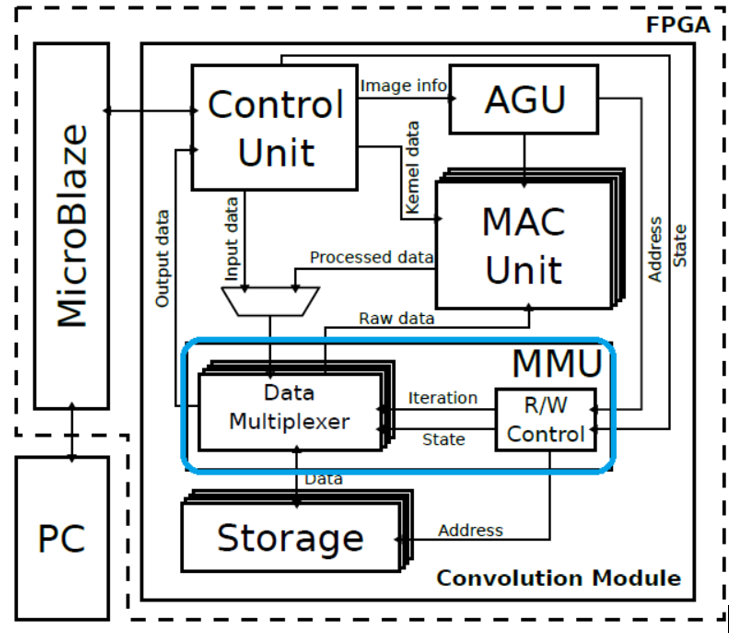
\includegraphics[scale=0.8]{arq_blue.png}
\caption{Bloque MMU}
\label{mmu_location}
\end{figure}

\bigskip
Analizando la arquitectura interna de los bloques que conforman este módulo, el bloque data multiplexer está conformado por un conjunto de bloques más pequeños clasificados en dos clases acorde a la función que cumplen:
\begin{frame}{}
\begin{itemize}

 \item \textbf{$MMB$(Memory Multiplexer Blocks)}
  \item \textbf{$PMB$(Processing Multiplexer Blocks)}

\end{itemize}
\end{frame}


Los $MMB$ hacen el routing de la información sin procesar (raw data) y la información desde las unidades $MAC$ hacia las memorias.
Los $PMB$ hacen el routing de la información desde las memorias hacia las unidades $MAC$.\\
\bigskip

Este flujo se puede ver en la siguiente figura:
\begin{figure}
\centering
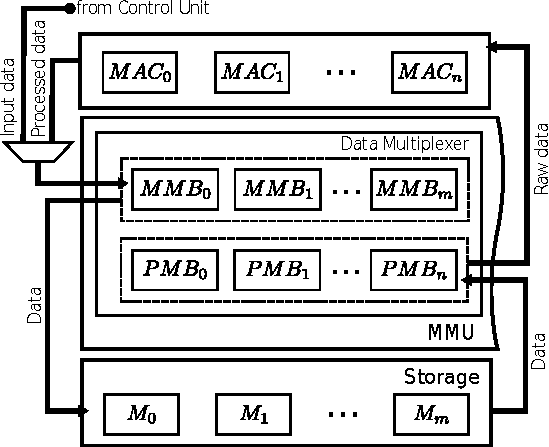
\includegraphics[scale=0.9]{muxes}
\caption{ Enrutamiento de información}
\label{mmu_routing}
\end{figure}
Tanto los bloques $MMB$ como los $PMB$ tienen un numero de entradas proporcional al numero de estados de la $FSM$ interna del bloque $MMU$. 
Las entradas a sus multiplexores se definen respectivamente:
\begin{equation}%\label{niter}
  O_j^i = O_{[(k-1)i+j]\%N}
\end{equation}
\begin{equation}%\label{niter}
  M_j^i = M_{(iN+j)\%(N+k-1)}
\end{equation}
\\
donde el símbolo $ \% $ representa la operación módulo, e $i$ toma valores desde $0$ a $It-1$.

\bigskip
\bigskip
\begin{figure}
\centering
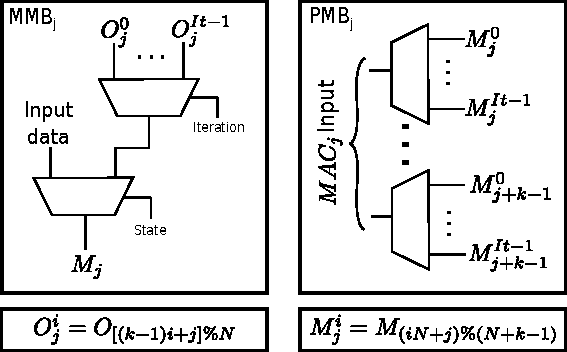
\includegraphics{muxes_cont}
\caption{ Estructura de los bloques MMB y PMB}
\label{mmu_structure}
\end{figure}